\documentclass[sigplan,screen]{acmart}

%%
%% \BibTeX command to typeset BibTeX logo in the docs
\AtBeginDocument{%
  \providecommand\BibTeX{{%
    Bib\TeX}}}

%% Rights management information.  This information is sent to you
%% when you complete the rights form.  These commands have SAMPLE
%% values in them; it is your responsibility as an author to replace
%% the commands and values with those provided to you when you
%% complete the rights form.
\setcopyright{acmcopyright}
\copyrightyear{2025}
\acmYear{2025}
\acmDOI{XXXXXXX.XXXXXXX}

%% These commands are for a PROCEEDINGS abstract or paper.
\acmConference[FUNARCH '25]{The Third ACM SIGPLAN Workshop on Functional Software Architecture -- FP in the Large}{October 17,
  2025}{Singapore}
%%
%%  Uncomment \acmBooktitle if the title of the proceedings is different
%%  from ``Proceedings of ...''!
%%
%%\acmBooktitle{Woodstock '18: ACM Symposium on Neural Gaze Detection,
%%  June 03--05, 2018, Woodstock, NY}
% \acmPrice{15.00}
% \acmISBN{978-1-4503-XXXX-X/18/06}


%%
%% Submission ID.
%% Use this when submitting an article to a sponsored event. You'll
%% receive a unique submission ID from the organizers
%% of the event, and this ID should be used as the parameter to this command.
%%\acmSubmissionID{123-A56-BU3}

%%
%% For managing citations, it is recommended to use bibliography
%% files in BibTeX format.
%%
%% You can then either use BibTeX with the ACM-Reference-Format style,
%% or BibLaTeX with the acmnumeric or acmauthoryear sytles, that include
%% support for advanced citation of software artefact from the
%% biblatex-software package, also separately available on CTAN.
%%
%% Look at the sample-*-biblatex.tex files for templates showcasing
%% the biblatex styles.
%%

%%
%% The majority of ACM publications use numbered citations and
%% references.  The command \citestyle{authoryear} switches to the
%% "author year" style.
%%
%% If you are preparing content for an event
%% sponsored by ACM SIGGRAPH, you must use the "author year" style of
%% citations and references.
%% Uncommenting
%% the next command will enable that style.
%%\citestyle{acmauthoryear}


%%
%% end of the preamble, start of the body of the document source.
\begin{document}

%%
%% The "title" command has an optional parameter,
%% allowing the author to define a "short title" to be used in page headers.
\title{Evolution of Functional UI Paradigms}

%%
%% The "author" command and its associated commands are used to define
%% the authors and their affiliations.
%% Of note is the shared affiliation of the first two authors, and the
%% "authornote" and "authornotemark" commands
%% used to denote shared contribution to the research.
\author{Markus Schlegel}
\email{markus.schlegel@active-group.de}
\affiliation{%
  \institution{Active Group GmbH}
  \streetaddress{Hechinger Straße 12/1}
  \city{Tübingen}
  \country{Germany}
  \postcode{72072}
}

\author{Michael Sperber}
\email{michael.sperber@active-group.de}
\affiliation{%
  \institution{Active Group GmbH}
  \streetaddress{Hechinger Straße 12/1}
  \city{Tübingen}
  \country{Germany}
  \postcode{72072}
}

%%
%% The abstract is a short summary of the work to be presented in the
%% article.
\begin{abstract}
  Functional paradigms for user-interface (UI) programming have
  undergone significant evolution over the years, from early
  monad-based approaches mimicking OO practice to modern
  model-view-update frameworks.  Changing from the inherently
  imperative classic Model-View-Controller pattern to functional
  approaches has significant architectural impact, drasticallyg
  reducing coupling and improving testability and maintainability.  On
  the other hand, achieving good modularity with functional approaches
  is an ongoing challenge.  This paper traces the evolution of
  functional UI toolkits along with the architectural implications of
  their designs, summarizes the current state of the art and discusses
  remaining issues.
\end{abstract}

%%
%% The code below is generated by the tool at http://dl.acm.org/ccs.cfm.
%% Please copy and paste the code instead of the example below.
%%
\begin{CCSXML}
<ccs2012>
   <concept>
       <concept_id>10010520.10010521</concept_id>
       <concept_desc>Computer systems organization~Architectures</concept_desc>
       <concept_significance>500</concept_significance>
       </concept>
   <concept>
       <concept_id>10011007.10010940.10010971.10010972</concept_id>
       <concept_desc>Software and its engineering~Software architectures</concept_desc>
       <concept_significance>500</concept_significance>
       </concept>
   <concept>
       <concept_id>10011007.10011006.10011008.10011009.10011012</concept_id>
       <concept_desc>Software and its engineering~Functional languages</concept_desc>
       <concept_significance>500</concept_significance>
       </concept>
 </ccs2012>
\end{CCSXML}

\ccsdesc[500]{Computer systems organization~Architectures}
\ccsdesc[500]{Software and its engineering~Software architectures}
\ccsdesc[500]{Software and its engineering~Functional languages}

%%
%% Keywords. The author(s) should pick words that accurately describe
%% the work being presented. Separate the keywords with commas.
\keywords{functional programming, software architecture, education}
%% A "teaser" image appears between the author and affiliation
%% information and the body of the document, and typically spans the
%% page.
\received{1 June 2023}

% FIXME revise

%%
%% This command processes the author and affiliation and title
%% information and builds the first part of the formatted document.
\maketitle

\section{UI and Software Architecture}

FIXME: basic terminology and thesis

% coupling, modularity

\section{Model-View-Controller}

% http://bildungsgueter.de/Smalltalk/Pages/MVCTutorial/Pages/FS0004.htm

The most prominent early example for the design of UI programs and
toolkits is Trygve Reenskaug's \textit{Movel-View-Controller} pattern
(MVC)~\cite{MVC}.  The central innovation of MVC idea was the
decoupling of UI code (``view'') from the domain logic (``model''),
with the specific intent of allowing multiple different views on the
same model.

MVC is---at least nominally---the ancestor of most contemporary UI
paradigms and frameworks.  The separation of the model from the view
is universally beneficial from an architectural standpoint.
Developers can change the UI and replace the UI toolkit without
changing the model.  Moreover, since the model can function without
the UI, testing automation is significantly easier compared to a
tightly coupled view.  (If the only way to manipulate the model is
through the UI, automated tests need to remote-control the UI, which
is tedious to implement and brittle.)

MVC programs need to keep the view current when the state of the model
changes.  To that end, models typically implement a variation of the
\textit{observer pattern}~\cite{GoF}: The model maintains a list of
``dependents,'' i.e.\ objects that it notifies on changes by calling
an \texttt{update:} method.  (The controller is tightly coupled to the
view, and its role is unimportant for this discussion.)

As the \texttt{update:} method informs the view of state changes, this
approach is inherently imperative.  MVC has nice modularity
properties, as each part of the model only needs to be coupled to
``its'' part of the view.  It also creates several challenges to
software architects:
\label{sec:challenges}
%
\begin{enumerate}
\item Keeping the view current with respect for the model involves two
  tasks: initially \emph{constructing} the view by creating the
  various UI widgets, and later \emph{mutating} the view upon calls to
  \texttt{update:}.  Conceptually, the result of mutating the view
  should be the same as re-constructing the view, but the concrete
  code for both is quite different, implementing the same logic twice.
\item To achieve modularity, architects should like to split a large,
  complex view into loosely coupled subviews.  This raises the
  question of how big those subviews should be. Making them large and
  correspondingly having them represent a largher chunk of the model
  simplifies the change logic, as it requires fewer implementations of
  \texttt{update:}, However it also increases coupling between model
  and view.  Moreover, it causes potential performance issues when the
  typical change is only to a small part of the model and only needs a
  small part of the view to change: In that case, \texttt{update:}
  either spends time drilling down to this small part of the view or
  changing larger parts of the view than necessary.
\item The view is not just a passive display, but will typically
  include interactive elements that cause changes in the model.
  Naively implemented, these changes indirectly trigger calls to
  \texttt{update:} in the view, which again might spill over into
  changes, causing a cyclic call chain.
\end{enumerate}
%
Consider the following practical example:
%
% weather composite, air pressure, temperature controls

\begin{figure}[tb]
\begin{verbatim}
class Weather(field pressure: Pressure,
              field temperature: Temperature) {
}

interface Observer {
  method update(info)
}

class Model {
  var observers: List Observer

  method changed(info) {
    for each sobserver in self.observers
      observer.update(info)

  method subscribe(observer) {
    observers += observer
  }
}

class Pressure extends Model {
  var hPa: double
  method setHPa(newHPa: double) {
    self.hPA = newHPa
    self.changed(newHPA)
  }
}

class Temperature extends Model {
  var kelvin: double
  method setKelvin(newKelvin: double) {
    self.kelvin = newKelvin
    self.changed(newKelvin)
  }
}
\end{verbatim}
  \caption{Model for weather data}
  \label{fig:weather-model}
\end{figure}

\begin{figure}[tb]
\begin{verbatim}
class TemperatureView
  (field temperatureModel: Temperature):
{
  var textField =
    new TextField(toText(temperatureModel.kelvin) + "K")

  temperatureModel.subscribe(self)

  method update(newKelvin) {
    textField.setText(toText(newKelvin) + "K")
  }
}

class PressureView
  (field pressureModel: Pressure)
{
  var textField =
    new TextField(toText(pressureModel.hPa) + "hPa")

  pressureModel.subscribe(self)

  method update(newHPa) {
    textField.setText(toText(newKelvin) + "hPa")
  }
}

class WeatherView(field weatherModel: Weather) {
  var temperatureView =
    new TemperatureView(weatherModel.temperature)
  var pressureView =
    new PressureView(weatherModel.pressure)
  ...
}
\end{verbatim}
  \caption{View for weather data}
  \label{fig:weather-view}
\end{figure}
%
Figure~\ref{fig:weather-model} shows object-oriented pseudcode for a
weather model that contains air pressure and temperature, each with
its own encapsulated state.  Figure~\ref{fig:weather-view} shows
skeleton code for a view that displays both in text fields.  The code
demonstrates nicely the modularity of the approach, as
\texttt{PressureView} and \texttt{TemperatureView} each subscribe to
their respective models, with no coordination required from
\texttt{WeatherView}.

The example also illustrates the first two challenges explained above:
%
\begin{enumerate}
\item The code for constructing the string representing the pressure
  and temperature is duplicated between the code that constructs the
  text field and the code that updates it.  It is possible to abstract
  out some code, but the fundamental separation between construction
  and update---which have to be consistent---remains.
\item The code contains two sub-views, updated separately.
  Alternatively, the subscription and update could happen between
  \texttt{WeatherView} and \texttt{Weather}, reducing modularity
  somewhat but also reducing the amount of code required.
\end{enumerate}
%
Note that the views are missing code to unsubscribe them from their
respective models---this further complicates the interaction between
model and view.

\begin{figure}[tb]
\begin{verbatim}
class TemperatureView2
  (field temperatureModel: Temperature) {
  var celsiusView =
    new TextField(toText(kToC(temperatureModel.kelvin)))
  var fahrenheitView =
    new TextField(toText(kToF(temperatureModel.kelvin)))

  temperatureModel.subscribe(new Observer {
      method update(newKelvin) {
        celsiusView.setText(toText(kToC(newKelvin)))
    }
  })
  temperatureModel.subscribe(new Observer {
      method update(newKelvin) {
        textField.setText(toText(kToC(newKelvin)))
    }
  })
  celsiusView.subscribe(new Observer {
     method update(...) {
      temperatureModel.setKelvin(cToK(...))
     }
  })
  fahrenheitView.subscribe(new Observer {
     method update(...) {
      temperatureModel.setKelvin(fToK(...))
     }
  })
}
\end{verbatim}
  %
  \caption{Two different sub-views on the same model}
  \label{fig:temperature-view2}
\end{figure}
%
Figure~\ref{fig:temperature-view2} shows a different view, just on the
temperature, but with two sub-views showing the temperature with
different units.  The code also adds the element of interactivity:
When the user interacts with the view, the two observers attached to
the views update the model.  This demonstrates the third challenge
described above: There is now an update loop between the model and
the two views: Each update to the model updates the view, which
updates the model, and so on.  The code could break the loop by
checking whether the new value is different from the old before
calling \texttt{changed}, but this is brittle---especially as
floating-point rounding is involved in the conversion between the
three units.

\section{The Curse of the Event Loop}
\label{sec:event-loop}

MVC UI toolkit also face a recurring implementation challenge: While a
MVC program constructs the UI in terms of hierarchically organized
views, it must display the UI as flat panel of pixels.  This means
that technically users interact with the UI panel as a whole, and the
UI toolkit must infer the view that is the target of the interactions.
Consider for example a button, which the user presses by clicking with
a mouse: The UI toolkit must infer from the position of the mouse
cursor the particular button view at those coordinates, and cause its
subscribers to be notified.

UI toolkits have traditionally chosen to implement this process using
an \textit{event loop}, a piece of code that receives hardware input
events and calls subscriber callback of the corresponding
views.  This happens repeatedly \textit{ad infinitum}, hence the
``loop''.  Here is pseudocode for a typical event loop:
%
\begin{verbatim}
while (true) {
  var event = get_input_event()
  dispatch_event(event)
}
\end{verbatim}
%
For this to work in practice, the \textit{update} methods of the view
subscribers must not block, as this would prevent further user
interaction.  If an \textit{update} method needs to perform I/O or
other blocking operations, this restriction effectively inverts the
flow of control: The method must start the operation asynchronously
and register it with the event loop, to be notified when the operation
has completed.  This is often awkward---more so, when the event loop
of a particular UI toolkit only supports a limited set of such
operations, as is common.

In principle, UI programs could also just start threads that perform
blocking operations synchronously, but interact with the UI
asynchronously.  However, many UI toolkits insist on their functions
being called from the thread the UI toolkit runs in, further
complicating matters.

Thus, typical MVC UI toolkits would couple the control flow of the
central event loop to the control flow of the subscriber callbacks,
which includes the code that manipulates the model.  The restrictions
resulting from this coupling often force developers to write these
callbacks and their dependencies in a non-linear arrangements,
creating a style of programming colloquially known as \textit{callback
  hell}.

\section{Functional UI Toolkits: The Early Days}

This section briefly describes some early UI tookits for functional
languages.  We focus on toolkitts that implemented genuinely
functional ideas.  Many other UI toolkits for functional languages
basically provided bindings for underlying C/C++ libraries and thus
inherited its imperative MVC pattern.

\subsection{eXene}

The eXene~\cite{eXene} toolkit was developed as part of the Concurrent
ML project~\cite{ConcurrentML} (CML).  CML is a combinator library in
Standard ML for arbitrarily assembling communication events.  EXene
uses Concurrent ML to solve the event-loop problem described in
Section~\ref{sec:event-loop}.  In eXene, the global event loop is
relegated to the background in favor of individual event loops running
in threads, each associated with a UI widget.  Rather than calling
subscriber methods directly, the event loop sends asynchronous
messages to the widget event loops.  This decouples the control flow
of the central event loop from that of its components.  Implementors
of components are afforded great flexibility in orchestrating their
actions through CML's event combinators.

While CML and eXene originated in the context of functional
programming, and CML's combinators rely on higher-order functions to
some extent, the overall approach of UI manipulation in eXene remains
firmly imperative.  Thus, eXene inherits challenge \#1 from Section~\ref{sec:challenges}.

\subsection{Fudgets}

While Standard ML is (also) an imperative language, Haskell is pure.
Haskell's lazy evaluation makes just adding functions that ``do
stuff'' impractical.  Consequently, interacting with the outside world
was generally a challenge for the designers of Haskell during its
nascency in the 1990s.  This also affects the designers of UI
libraries who were motivated to specify UIs in terms of pure
functions.  A notable early attempt to do this was the
\textit{Fudgets} toolkit~\cite{Fudgets}.  (At the time of writing,
Fudgets is still being maintained as a Haskell library.)

Fudgets represents a UI component (a \textit{fudget}) as a
\textit{stream processor} of type \verb|F a b| that transforms a
stream of input values of type \texttt{a} into output values of type
\texttt{b}.  Fudgets can be combined into sums and products, building
UI structure and reactivity in a hierarchical fashion.  Fudgets
completely abstracts the event-loop paradigm away from the user
program, which consists exclusively of pure functions.

The view of fudgets as attaching pure functions to laid-out UI
components implies that the structure of the fudgets is static.  UIs
frequently need to have dynamic structure, however---for example, when
displaying a list of UI items that supports adding and removing
elements.  Fudgets addresses this by combinators that accept special
command values that describe mutations of the UI structure,
effectively sneaking in imperative elements in its otherwise pure
model.  Thus, Fudgets also partially inherits challenge \#1 from
Section~\ref{sec:challenges}.

\subsection{Fruit}

Fruit~\cite{Fruit} re-imagines the basic idea of Fudgets on top of the
idea of Functional-Reactive Programming~\cite{FRP}, which had been
developed in the meantime.  Fruit retains the purity and
compositionality of Fudgets,  replacing the stream processors of
Fudgets with FRP signal transformers.  There are two notable
differences between Fudget and Fruit, however:
\begin{itemize}
\item Fudgets widgets have implicit access to interactive events,
  while Fruit requires them to be threaded explicitly through the
  program.  This means that a Fruit program is coupled to all aspects
  of the ``outside world'' it interacts with, making it difficult to
  add interactions outside the UI (such as file or network I/O) after
  the fact.
\item Another difference concerns dealing with dynamic UI components:
  Whereas Fudget views by default display the values coming from a
  stream (and are thus ``outside'' those streams), Fruit has the views
  themselves be the values of the FRP signals, and dynamic structure
  can be expressed by just having new values return a different view.
\end{itemize}
%
Thus, Fruit avoids challenge \#1 from Section~\ref{sec:challenges},
but comes with its own modularity problem.

\subsection{Haggis}

Haggis was a short-lived UI toolkit for GHC~\cite{Haggis}, which took
somewhat of middle path between eXene and Fudgets: While Fudgets
provides a purely functional UI for constructing widgets via explicit
combinators, Haggis provides an imperative UI running in the
\texttt{IO} monad for this construction.  Haggis deals with the event
loop similarly to eXene, replacing Concurrent ML with Concurrent
Haskell.  For the reactive part of a UI widget, Haggis provides a
handle separate from the view part.  The program can wait for
interaction on these handles also in the \texttt{IO} monad (in
separate threads if that is convenient), and allows combining them in
a way similar to CML events.  Thus, Haggis also inherits challenge
\#1 from Section~\ref{sec:challenges}.

\section{The Racket Universe Teachpack}
\label{sec:universe-teachpack}

Teachers of introductory programming courses would often like to
enable their students to write interactive programs.  The complexity
of UI toolkits have traditionally made this difficult, at least in the
era of toolkits described in the previous section.  The Racket system
comes with a library called the \textit{Universe teachpack} for an
introductory course~\cite{UniverseTeachpack} that allows writing
distributed, interactive video games in a purely functional manner.

The Universe teachpack is basically ``half'' a UI toolkit.  It is an
interesting subject for study, as it does address the pernicious
challenge \#1 of the UI toolkits described above: The duplication of
view logic between initial construction and later update.  We focus
here on the ``world'' part of the universe teachpack, i.e.\ video
games without distribution.  To implement such a video game, the
developer only has to implement a small number of pure functions, all
of which operate on a model called the ``world state,'' represented by
a single value of type \texttt{WorldSt}:
%
\begin{verbatim}
on-draw : WorldSt → Image
on-tick :  WorldSt → WorldSt
on-key :  WorldSt KeyEvt → WorldSt
on-mouse : WorldSt Nat Nat MouseEvt → WorldSt
\end{verbatim}
%
These functions are all callbacks for the Universe teachpack, the
programs contains no explicit calls to them.

The \texttt{on-draw} function handles view construction and uses Racket's
\texttt{image} teachpack to build a single frame of the video game.
(The \texttt{image} teachpack is a combinator library in the style of
Henderson's functional geometry~\cite{Henderson1982}.)  There is no
separate function for view \emph{update}: Whenever the model
transitions to a new state, the Universe teachpack simply calls
\texttt{on-draw} again and redraws the \emph{entire} frame.  This is
fast enough in practice to achieve reasonably fluid animation.

The other functions provide reactivity to different kinds of events:
All of them take a \texttt{WorldSt} state as input and output a new
state, which the teachpack feeds into \texttt{on-draw}.
\texttt{On-tick} is called on every clock tick to provide movement
even when there is no user interaction.  \texttt{On-key} is called on
key presses, and \texttt{on-mouse} on mouse events.  Writing these
functions is well within the purview of introductory-course students.

Consequently, the Universe teachpack uses a ``brute-force'' approach
to the view-update poblem: Use a single monolithic value for the model
state, and redraw everything every time the model moves to a new
state.  This means no separate view-update code---challenge \#1
solved.

Unfortunately, this approach also abandons the good modularity
properties of object-oriented MVC toolkits: From the point of view of
the UI toolkit, the model state is a single value, and there is no
simple way to split it---and the corresponding view elements---into
sub-views while retaining a similarly simple API.  Thus, the Universe
teachpack faces the sub-view challenge \#2 from
Section~\ref{sec:challenges}.  This is not a
problem in this context: The video games realistically implemented in
a video game are simple enough that unified state is appropriate.  It
does prevent easily scaling the approach to realistic UIs.

% Conal's UI paper
% http://conal.net/papers/Eros/
% PureScript/Halogen

\section{The Evolution of Elm and React}

Elm~\cite{Elm} is a UI toolkit and companion Haskell-like language
that translates to JavaScript and thus allows implementing web
applications.  Elm is in production use in quite a few open-source and
commercial projects.  Elm's initial release in 2012 was based on FRP Signals,
and was similar to Fruit.  Its innovation was its support for
asynchronous I/O, which is a problem for Fruit because of its global
approach to I/O.

Elm evolved to an approach different from that of its inception,
leaving its FRP legacy behind in 2016~\cite{ElmFarewellFRP}.  This approach
gives rise to an alternative UI pattern called
\textit{Model-View-Update}.  An Elm program mostly consists of only
two pure functions operating on values of a type \texttt{Model},
defined by the UI program:
%
\begin{verbatim}
view : Model -> Html Msg
update : Msg -> Model -> (Model, Cmd Msg)
\end{verbatim}
%
\begin{figure}
  \centering
  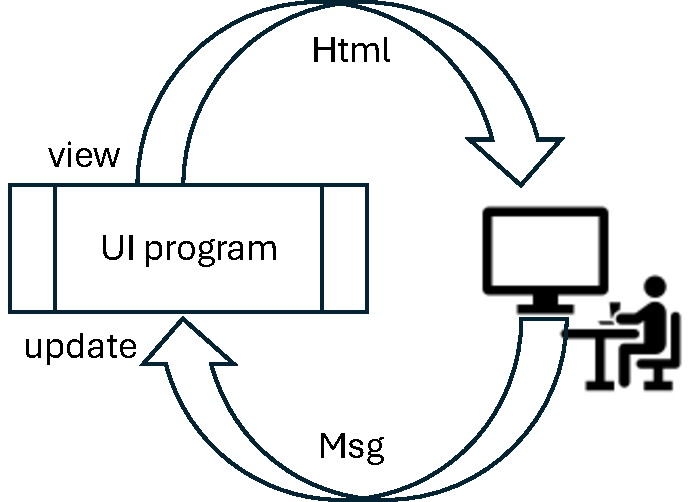
\includegraphics[width=\columnwidth]{model-view-update}
  \caption{The Model-View-Update pattern}
  \label{fig:mvu}
\end{figure}
%
Figure~\ref{fig:mvu} illustrates the pattern.
The \texttt{view} function constructs the UI, represented as a HTML
tree.  Each interactive UI widget carries a message of the
\texttt{Msg} type (also defined by the UI program) that is generated
when the user interacts with the widget.  The Elm toolkit than passes
this message to the \texttt{update} function that generates a new
model, which again gets fed into \texttt{view} and so on.  (The
\texttt{Cmd} type allows triggering impure actions outside of user
interactions.)

The View-Model-Update model is extraordinarily simple and easy to
learn, as it does not require the developer to know any higher-level
abstractions like signals, stream transformers or monads.  It also
completely avoids the circular dependency between view and model.

The idea of Model-View-Update is quite similar to that of Racket's
Universe teachpack: The view is re-constructed after every user
interaction, and it uses a single, monolithic value for the model
state.  The possible messages belong to a single central type.

Consequently, Elm also inherits the Universe teachpack's architectural
trade-offs: It solves challenge \#1 from Section~\ref{sec:challenges},
but has no notion of an
independent, composable ``UI component'' and thus faces challenge \#2.
Thus, achieving modularity
at the level of sub-models and sub-views is entirely up to the
developer.

Shortly after Elm's initial release, Facebook released their web UI
toolkit \textit{React}, which was also based on a variation of the
Model-View-Update paradigm.

React's \texttt{render} function corresponds to Elm's \texttt{view}
function: It transforms the model state into a HTML tree.  Unlike Elm,
React has a composable notion of a UI component---a sub-view with its
own associated state.  Consequently, \texttt{render} actually first
creates a tree of UI component, which then gets rendered into HTML.

Where Elm gives the UI program complete freedom in the choice of
\texttt{Model} type, React differentiates two kinds of state:
Immutable \textit{properties} that flow downward in the sub-view tree.
Each component also has its own associated mutable \textit{state},
which needs to be organized as a JavaScript hash map.
Thus, React's model of reactivity is different from Elm's: The UI
program attaches imperative callbacks to UI components, and these
callbacks can either mutate the component state or cause the
properties to be replaced.  Conceptually, React ignores the difference
between these two methods and re-renders the entire UI on each
interaction, just like Elm.  Over time, mutating the state became
recognized as an anti-pattern in the React community, and updating the
UI happens in a manner quite similar to Elm.

% FIXME: maybe notes on the implementation

Elm and React represented an erstwhile peak in the evolution of
functional APIs, intellectually hailing from Fudgets and Fruit, and
effectively rendering the functional toolkits that came before them
obsolete: The simplicity of the Model-View-Update paradigm makes it
attractive for a wide spectrum of developers---specifically, it
requires no deeper understanding of higher-level concepts such as
stream transformers, signals, or arrows.  Yet Model-View-Update is
powerful enough to enable even complex applications.  Consequently, we
take Model-View-Update as the starting point for the further
discussion of this paper.

% Redux?

\section{UI Toolkits Elsewhere}

\section{Functional Modularity Challenges}

Taking Elm's and React's Model-View-Update pattern as a starting
point, we summarize the architectural tradeoffs listed in
Section~\ref{sec:challenges}:
%
\begin{enumerate}
\item Model-View-Update solves challenge \#1: A single function
  describes view construction, no separate logic for view update is
  needed.
\item Implementing sub-views in a modular fashion remains a challenge:
  A functional Elm/React application essentially manages its model
  state as a single mutable reference at the top level, with
  everything below managed functionally.
\item Movel-View-Update also solves challenge \#3, as the cyclic call
  chain is broken by the sequences succession of models and updates
  presented to the UI toolkit.
\end{enumerate}
%
Solving challenge~\#2 in means establishing a notion of ``UI
component'' without resorting to imperative state updates.  A solution
approach needs to address facets described in this section: Updating
the model state in a modular fashion, dealing with UI-local state, and
breaking up global dispatch.

We will illustrate these facets using a simple example: Imagine an
application that manages phone-book entries with name and phone
number.  The application manages the phone book in a functional
manner, as a functional list of immutable entry records.  Its UI
contains a sub-view component that allows viewing and editing a single
name within a text field, along with a ``Submit'' button for actually
changing the address book.

% FIXME: maybe a figure

\subsection{Global Model State Update}

When the user changes the name, this is a local change from the point
of view of the UI component, but leads to a global change in the
application, which must update its phone-book reference.  So strictly
speaking, updating the state is not the job of the name UI component
but of all the components above it in the hierarchy that need to
re-construct the state with the one changed name, and finally change
to global reference at the top.

\subsection{UI-Local State}

The model-state update happens when the user clicks the ``Submit''
button.  However, the UI carries state even before that, as the user
types in the new name, usually one letter at a time.  The UI toolkit
must manage this ``UI-local'' state.  However, as it is an artifact of
the UI widget and not an aspect of the model, the UI toolkit should
enable separting them.

Note that the classification between model state and UI-local state
depends on context and judgement: The name UI component itself has two
sub-components, a text field and the submit button.  The text field's
model will usually be the visible text.  However, embedded within the
name component, the text field's model state becomes the name
component's UI-local state.

\subsection{Global Dispatch}

In Elm, the UI program communicates requests to change the model state
(as well as other side effects) via messages of type \texttt{Msg},
which the toolkit subsequently passes to the \texttt{update} function.
This \texttt{update} function is global, and thus unmodular.  Making
the global dispatch modular requires associating it with an individual
UI component rather than the program as a whole.

However, a UI component is often not able to handle the messages
generated user interaction with its view.  Consider again the name UI
component: The name should probably not be empty, and thus the
``Submit'' should be deactivated as long as the text field is empty.
Thus, the text-field component must, pass a message upwards to its
enclosing name component informing it of the state change.
Correspondingly, the enclosing component must be able to handle the
message coming up from its sub-component.

Furthermore, the type of the message produced by the sub-component
must match the type expected by the enclosing component.  This is not
necessarily the case when the two are developed separately: For this
case, the UI toolkit must offer a mechanism to transform the message
along the way from its producer to its handler.

\section{From Model-View-Update to Reacl}


\section{Persistent Pains}

User interface construction remains a struggle. In addition to
challenges described above, UI programming -- and testing -- is
considered difficult for reasons that are beyond the grasp of UI
frameworks and libraries.

\subsection{Inherently vague semantics}

Many functional user interface frameworks and libraries claim that
they allow users to describe their UI as a pure function from state
(domain model) to a description of a graphical display -- for example
HTML. According to FP folklore, pure functions are easy to
test. Consequently, it should be easy to write UI tests: Run the
function \texttt{f} that is your UI for a sample \texttt{state} of
your domain logic and compare the resulting graphical display
\texttt{(f state)} to your desired version. Even if we forget about
the dynamic nature of UIs for a moment, this approach rarely results
in good tests. Take this temparature display in pseudo-code:
%
\begin{verbatim}
  // a user interface
  let f temp
    = <div
        style={if (tooHot temp)
                 "background: red;"
               else
                 ""}>
       {string_of_temp temp}
      </div>

  // test
  assertEqual (f 22) <div>22</div>
  assertEqual (f 183) <div style="background: red;">183</div>
\end{verbatim}
%
This trivial test already misses the mark. Say we are dissatisfied
with a red background color but we still want to emphasize
temperatures that are too hot. It is reasonable to assume that a red
border is sufficient to fulfill that need. Our test, however, is of a
different opinion. Our test demands backgrounds to be red. In these
situations we have to adapt both our implementation \textit{and} our
tests. This is fine if \textit{these situations} happen rarely. In UI
programming, they happen more often than not.

Tests show their merit under the evolution of implementations. A good
test checks whether an implementation satisfies a given interface,
while allowing for many different implementations. The interface of
most UI components is hard to separate from the implementation,
however. In the example above we want to ensure ``emphasis'', which as
an abstract concept is hard to formalize. Much of what it takes for an
user interface widget to be considered emphasized is out of reach for
its own graphical display: For one, user's habits and expectations
change constantly. A graphical representation that is perfectly
emphatic today might have been overlooked ten years ago. Additionally,
context plays an important role. A graphical representation that is
perfectly emphatic when surrounded by white space appears too timid
surrounded by loud advertisements.

\cite{SPE} suggests a classification of software programs into classes
\textit{S} -- ``programs whose function is formally defined by and
derivable from a specification'' --, \textit{P} -- programs that have
a formal specification, but ``the acceptability of a solution is
determined by the environment in which it is embedded.''  --, and
\textit{E} -- ``programs that mechanize a human or societal
activity''. Classes \textit{P} and \textit{E} are further aggregated
to form the class \textit{A} -- programs ``that represent a computer
application in the real world''. The distinction between \textit{S}
and \textit{A} programs aligns with our distinction between software
aspects that have a precise formal semantics and vague aspects like
\textit{emphasis}. \textit{S} programs are amenable to automated tests
or even formal verification. While it requires effort to write tests
or proofs, running automated tests or checking proofs is
cheap. \textit{A} programs on the other hand require manual tests to
verify their correctness. Running manual tests regularly is expensive
and may be totally infeasible for some software projects.

While most UI software falls into the \textit{A} class \textit{in its
  entirety}, large software is made from smaller parts, which in turn
can be classified as either \textit{S} or \textit{A}. In the
temperature display example above, we already identified
\textit{emphasis} as the problematic aspect in terms of precise formal
semantics -- an \textit{A} aspect. In contrast, the function
\texttt{tooHot} solely operates in terms of the core domain
logic. This function is independent of its context or any human habits
or practices. It belongs to class \textit{S}, and is therefore
amenable to automated tests and verification.

In order to bring down overall costs for tests, we have to strive for
a surgically precise discernment of \textit{S} software parts and
\textit{A} software parts. In other words: We want to write as little
UI code as possible. In the remainder of this work we propose a
discipline that supports this goal: we introduce reacl-c, a UI
combinator library that is optimized for reusability and we make an
argument for the \textit{functional view model}, a UI programming
pattern.

%% While the inherent vagueness in UI requirements prevents \textit{some
%%   aspects} of our UI code to be checked by automated tests, this
%% doesn't mean we have to resort to manual testing \textit{for every
%%   aspect of our UI code.} In the temperature display above, the
%% function \texttt{tooHot} solely operates in terms of the core business
%% logic and is therefore amenable to automated testing. In this small
%% example, the border between code that caters to vague requirements
%% vs. code that caters to formal requirements happens to align with the
%% border between UI code and business logic.  With the help of the
%% ``View Model'' pattern and UI programming models that allow for
%% fine-grained modularity we can push the border separating testable and
%% untestable code further into the UI part.

\section{From Reacl to reacl-c}

Reacl improves on its predecessors in terms of modularity. Modularity
is a neccessary prerequisite for reusability, but it is not
sufficient. Reacl often makes it hard to extract and reify certain
aspects of user interfaces, limiting reusability. This is primarily
due to the fact that Reacl requires early binding of state by
default. This means that when a user creates a new instance \texttt{C}
of a Reacl component, they have to decide then and there which other
component's state \texttt{C}'s state relates to and in which way. In
most cases, and as you can see in the examples above, the ``other
component'' is \texttt{this}, which is the conventional name for the
instance of the component that is being constructed at the current
moment. This pattern goes a long way. However, early binding of state
is at odds with the creation of custom component combinators. The lack
of custom combinators means untapped reuse potential.

%% This lack in expressivity lead to the creation of reacl-c. reacl-c provides a set
%% of UI primitives called items and a set of item combinators. Items
%% generally have a graphical appearance, may have controlled effects and
%% may return values to their context via so called
%% \textit{actions}. Additionally, since lots of UIs have a notion of
%% state, this notion is built in to reacl-c, even though it could
%% theoretically be implemented in terms of the other concepts.

reacl-c only targets web UIs at the moment. The reacl-c web UI
primitives and combinators are found in the \texttt{reacl-c.dom}
namespace.
%
\begin{verbatim}
  (require reacl-c.dom :as dom)
\end{verbatim}
%
These DOM items and item combinators only have a visual
appearance. They don't issue any effects or actions. They aren't
affected by state. An example for a DOM item constructor is
\texttt{span}, which takes a string and produces an item that, when
shown on screen, displays the given string inside a
\texttt{<span></span>} element. We can run reacl-c items with
\texttt{reacl-c.main/run} which takes an item to run and a DOM node.
%
\begin{verbatim}
  (require reacl-c.main :refer [run])

  (run (.getElementById js/document "main")
       (dom/span "Hello World"))
\end{verbatim}
%
The \texttt{reacl-c.dom} namespace also provides a set of item
combinators such as \texttt{div}, which takes an arbitrary number of
items and wraps their graphical appearances in a
\texttt{<div></div>}. All DOM items optionally take an attribute map
as a first argument. Item attributes usually correspond to DOM
attributes, so attribute maps are a way to style items. Note that
strings are also valid items that appear as themselves.
%
\begin{verbatim}
  ;; an item displaying "Hello " next to "World" in blue.
  ;; both words are surrounded by a green border.

  (dom/div
   {:style {:border "1px solid green"}}
   "Hello "
   (dom/span
    {:style {:color "blue"}}
    "World"))
\end{verbatim}
%
DOM items can issue actions or state changes via the \texttt{onClick}
attribute for example.

...



\subsection{The View Model -- functionally}


%%
%% The next two lines define the bibliography style to be used, and
%% the bibliography file.
\bibliographystyle{ACM-Reference-Format}
\bibliography{funarch-ui}

\end{document}
\endinput
%%
% TODOs:
% - cite Conal


